\section{\Klang{} In Practice}
\label{sec:usage}

Currently, \Klang{} is used to analyze models created for the
NASA Europa Clipper Mission. Figure~\ref{fig:k} gives an overview of
the usage scenarios for the \Klang{} language and tool chain.

\begin{figure*}
\centering
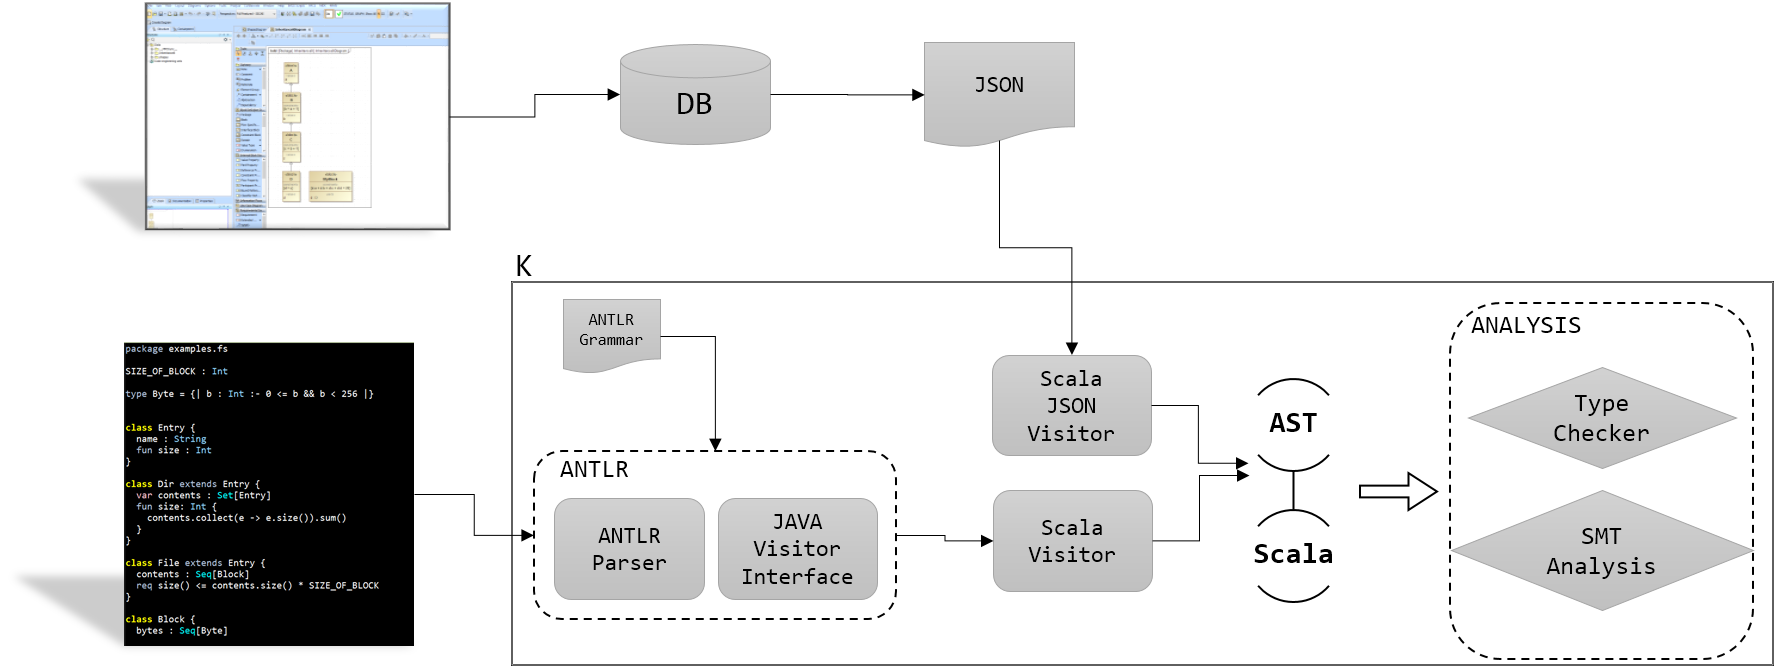
\includegraphics[scale=0.39]{K.png}
\caption{\Klang{} in practice.}
\label{fig:k}
\end{figure*}

The typical scenario involves modelers creating SysML diagrams in a
tool such as MagicDraw and saving them to a central model
repository. This database of models is accessible via a REST API. The
input to the REST API is a unique identifier for a node (typically a
\sysml{} package) in the model, and the result is a list of all the
nodes that are part of the package specified in the input. The result
is provided as an array of JSON objects, where each object contains
information such as name, type, owner, etc. Typically, the types of
objects are classes, constraints, expressions, and member
properties. The \Klang{} tool chain takes this input and converts each
node in the list of nodes to a corresponding \Klang{} AST
object. Since the list of nodes received from the REST API is
unordered and unstructured, we perform multiple passes on
the list of nodes. The first pass is performed to create the list of
classes in the model, followed by passes to populate properties and
constraints in each class. Once the \Klang{} model has been
constructed, the \Klang{} tool chain proceeds normally with type
checking and SMT analysis. Currently this scenario is based on a {\em
  pull} methodology where a modeler has to initiate the \Klang{} based
translation and analysis. In the future, we plan on automating this
effort and have it be executed on a regular cadence with results made
available through the model database to a web application.

\begin{figure*}
\centering
\fbox{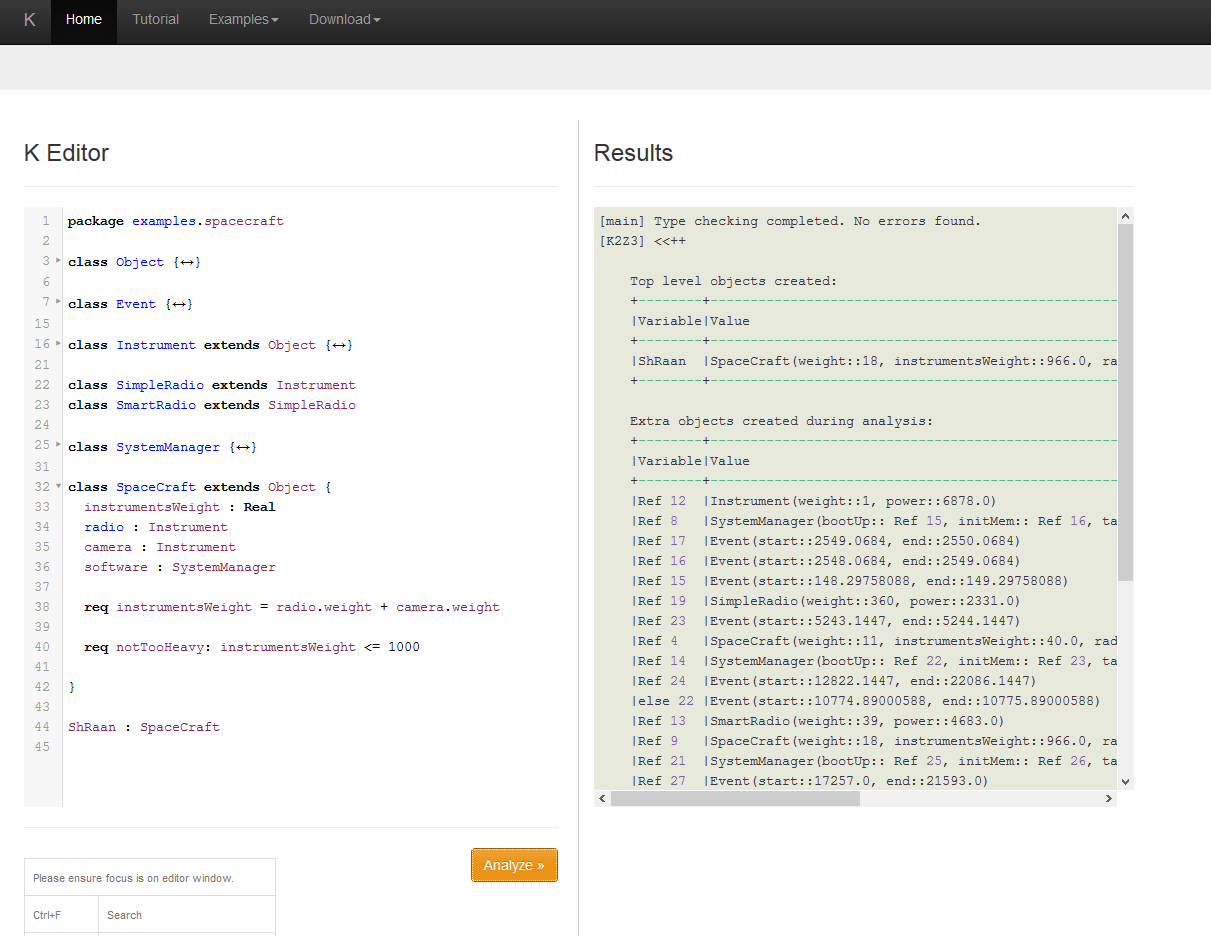
\includegraphics[scale=0.3]{kweb.png}}
\caption{\Klang{} editor in the browser.}
\label{fig:k}
\end{figure*}

A second common scenario for using \Klang{} is via the web browser. We
have created a simple HTML based \Klang{} code editor along with the
functionality to invoke the type checker and SMT analysis from the web
browser. This page is used for purposes of teaching, learning,
exploring, and prototyping with \Klang{}. The web page also provides a
tutorial, documentation, and \Klang{} examples as a guide. 

Finally, the \Klang{} tool chain is also available as a binary
download for all major operating systems. Users may download the tool
chain and invoke the \Klang{} parser, type checker, and SMT analyzer
from the command line.

